\chapter{Gestión y planificación del proyecto}

\section{Metodología}

En los primeros años del desarrollo de software, este se creaba sin seguir ningún enfoque formal. Muchos de los proyectos que se iniciaban terminaban fracasando por los retrasos en la entrega, el mal funcionamiento del producto o por no cumplir los requisitos del cliente. Además, la complejidad requerida en el software iba aumentando con el tiempo. 

Por ello, era necesario crear un marco que permitiera metodizar el desarrollo. Es así como surge la Ingeniería del Software, que acompaña al software durante todo su ciclo vital.

En este proyecto se va a aplicar este enfoque a la hora de desarrollar el producto, apoyándome sobre una metodología de desarrollo para asegurarnos que se consiguen los objetivos en el tiempo previsto, detectando posibles amenazas y problemas a tiempo.

Las metodologías se pueden clasificar en dos grandes bloques \cite{metodologiasDesarrollo}, tradicionales y ágiles. Las tradicionales son las que primero surgieron, se caracterizan por definir rígidamente los requisitos al inicio del proyecto. En ellas, se aplica una serie de etapas de forma lineal, y una vez alcanzada una de ellas no se puede volver atrás. Por todo esto no se adaptan bien a los cambios.

En general, los proyectos de software tienden a ser cada vez más complejos. Las metodologías ágiles surgieron con el objetivo de hacer los proyectos de desarrollo más dinámicos, de forma que se adaptaran mejor al entorno y a los cambios. Se basan en una metodología incremental, donde se van construyendo prototipos del producto poco a poco, añadiendo funcionalidades hasta obtener la aplicación final. Los equipos se reúnen cada poco tiempo para intercambiar ideas y repartir las tareas a realizar.

A la hora de elegir la metodología que se va a utilizar, se deben tener en cuenta los siguientes factores relativos a la naturaleza del proyecto:

\begin{itemize}
    \item Se trata de un proyecto de investigación, donde se van a aplicar diferentes técnicas de Aprendizaje Automático a la resolución de un problema. Por tanto, a priori no se conoce la calidad de los resultados que se van a obtener y el número y tipo de experimentos que va a ser necesario realizar.
    \item La intervención del experto en química va a ser fundamental durante el desarrollo del proyecto. Aportará información y feedback esencial durante todas las fases.
\end{itemize}

Por estas razones, creo que la metodología de desarrollo que mejor se adapta a nuestras necesidades es una metodología ágil, ya que nos provee de gran flexibilidad, permitiendo el desarrollo del proyecto de una forma incremental donde obtengo feedback del cliente y experto en cada iteración.

Revisando las distintas metodologías \cite{despa2014comparative}, creo que una buena candidata es SCRUM. Es posiblemente una de las más utilizadas en la actualidad, y los proyectos que la aplican cuentan con las siguientes características \cite{schwaber1997scrum}:

\begin{itemize}
    \item \textbf{Entregable flexible:} Su contenido viene dado por lo que demanda el entorno. 
    \item \textbf{Calendario flexible:} El entregable puede ser requerido antes o después de lo previsto.
    \item \textbf{Equipos pequeños:} Los equipos están formados por pocas personas, de forma que la comunicación y sincronización entre sus miembros es alta. 
    \item \textbf{Revisiones frecuentes:} El progreso del equipo se evalúa de forma periódica y frecuentemente, de forma que se ponen en común las dificultades encontradas y se intentan resolver con la ayuda de todos los miembros.
    \item \textbf{Colaboración:} La colaboración entre todos los miembros del equipo es muy alta, así como entre el equipo y entidades externas como el cliente.
\end{itemize}

Cuando se trabaja con esta metodología, en cada equipo existe un miembro conocido como SCRUM manager. Es el encargado de guiar al equipo en el desarrollo y en la aplicación de la metodología. En SCRUM el equipo es muy importante y todos sus miembros participan con su opinión. Esta metodología consta de las siguientes fases \cite{schwaber1997scrum}:

% TODO: Si fuera necesario, añadir información sobre los tipos de equipos. En el paper de SCRUM aparece información sobre estos.

\begin{figure}[H]
\centering
    \fbox{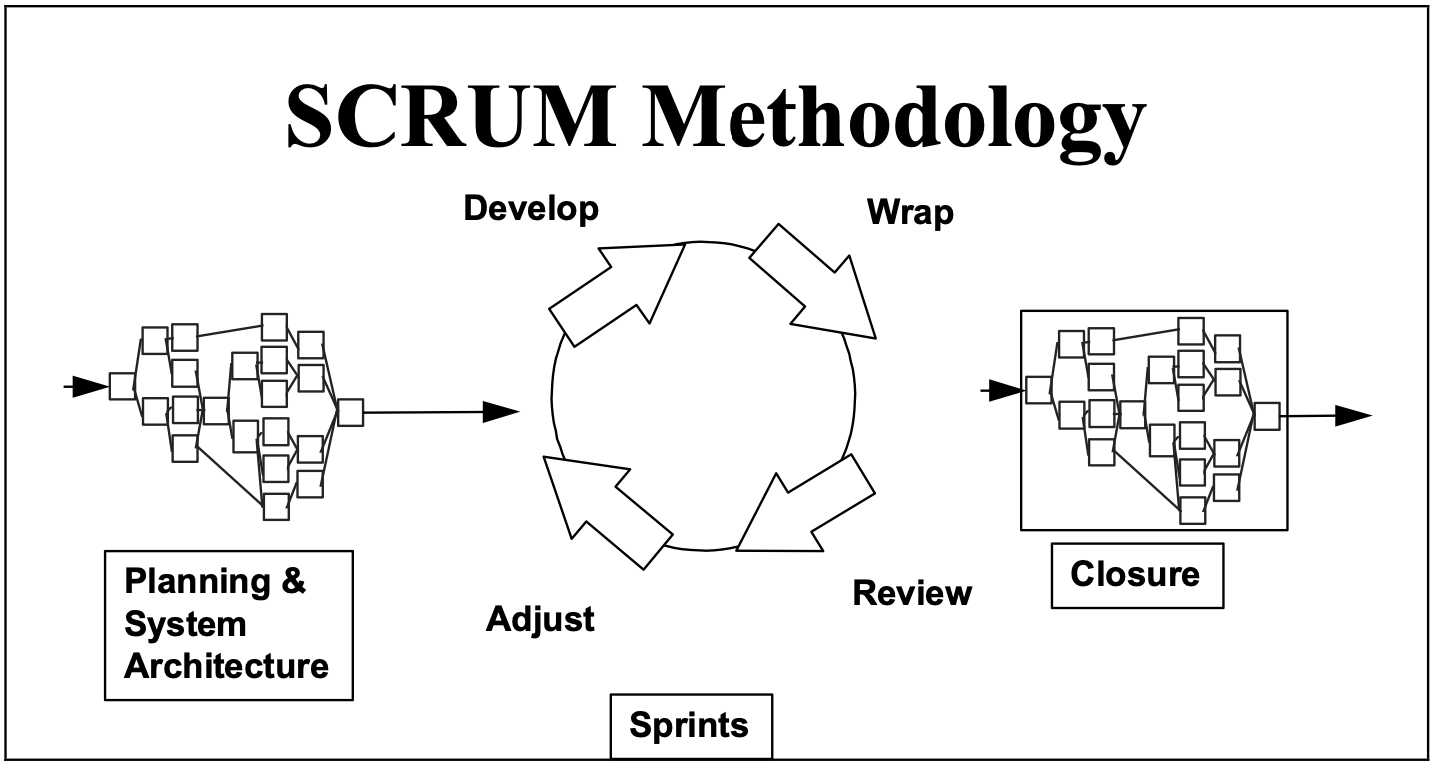
\includegraphics[scale=0.45]{imagenes/scrum.png}}  
    \caption{Fases de la metodología SCRUM \cite{schwaber1997scrum}} \label{fig:figura1}
\end{figure}

\begin{itemize}
    \item \textbf{Pregame:} 
    \begin{itemize}
        \item \textit{Planificación:} En esta fase se crea la lista de tareas a realizar (backlog list), se fija la fecha de entrega del producto y su funcionalidad, se forma el equipo (o equipos) de trabajo, se valoran los riesgos que puedan surgir, los costes y finalmente se revisa todo y se aprueba el proyecto.
        \item \textit{Arquitectura/Diseño de alto nivel:} Se revisan los elementos en el backlog, se realizan cambios si es necesario para poder implementarlos, se perfila la arquitectura del sistema teniendo en cuenta estos cambios y una reunión es organizada para revisar el diseño, donde cada equipo presenta una propuesta para implementar cada backlog.
    \end{itemize}
    \item \textbf{Game:} Corresponde con el conocido Sprint de la metodología SCRUM. Es la parte iterativa de la metodología, que se ejecuta varias veces hasta conseguir el producto final y está formada por las siguientes subtareas:
    \begin{itemize}
        \item \textit{Desarrollo:} Lo primero que se realiza es definir los cambios que hay que realizar en los backlogs para poder implementarlos. Se dividen las tareas presentes en el backlog en paquetes, y se completan estos paquetes diseñando, desarrollando, implementando, testeando y documentando los cambios.
        \item \textit{Envoltura:} Se cierran los paquetes, creando una ejecutable que incorpora los cambios y se explica como cumplen lo especificado en los backlogs.
        \item \textit{Revisión:} Todos los equipos se reunen para presentar el trabajo. El desarrollo obtenido se evalúa y se añaden nuevas tareas que puedan surgir al backlog. Se evalúa el riesgo y se realizan propuestas en base a este.
        \item \textit{Ajuste:} Se consolida la información recibida durante la revisión.
    \end{itemize}
    
    \item \textbf{Postgame:}
    \begin{itemize}
        \item \textit{Cierre:} Cuando el gestor del proyecto considera que el producto está terminado y cumple con los requisitos solicitados por el cliente se entra en esta fase, donde se prepara el producto para su despliegue. Integración, generación de la documentación, testeo y marketing son algunas de las actividades que se realizan en este paso.
    \end{itemize}

\end{itemize}

Estas características y fases que hemos mencionado son las especificadas en la definición original de SCRUM. Aún así, en la práctica cada proyecto las adapta a sus necesidades. En general, los sprints suelen tener una duración de 2 o 3 semanas. 

\section{Planificación} \label{planificacion}
Para lograr cumplir con los objetivos, se planifican las siguientes tareas a realizar:
\begin{itemize}
    \item \textbf{[T1]} Estudio del estado del arte del problema.
    \begin{itemize}
        \item \textbf{[T1.1]} Lectura de publicaciones introductorias a las Cheminformatics.  
        \item \textbf{[T1.2]} Repaso de la literatura sobre aprendizaje profundo, comprendiendo los principales modelos de generación y clasificación de imágenes.
        \item \textbf{[T1.3]} Conocimiento de las principales herramientas que se han desarrollado en ambos ámbitos.
    \end{itemize}
    \item \textbf{[T2]} Estudio del \textit{dataset} de imágenes químicas existente para su adecuación a tareas de clasificación.
    \begin{itemize}
        \item \textbf{[T2.1]} Mejorar el balanceo del \textit{dataset}.
        \item \textbf{[T2.2]} Adaptación de un modelo de síntesis de imágenes para generar \textit{hard negatives} y añadirlos al \textit{dataset}, de forma que el clasificador sea capaz de trabajar con ejemplos difíciles.
    \end{itemize}
    \item \textbf{[T3]} Implementación de dos modelos clasificadores de imágenes, capaces de distinguir moléculas de ejemplos negativos, uno entrenado sobre un \textit{dataset} sin \textit{hard negatives} y otro entrenado sobre un conjunto de datos con ellos.
    \begin{itemize}
        \item \textbf{[T3.1]} Realizar pruebas con diferentes arquitecturas e hiperparámetros para comprobar cuáles se adaptan mejor al problema.
        \item \textbf{[T3.2]} Escoger la configuración que tendrán los modelos finales. 
    \end{itemize}
    \item \textbf{[T4]} Documentación del trabajo realizado.
\end{itemize}

Para el éxito del proyecto es necesario asignar una temporización razonable a cada tarea. Este se realiza en el marco de un Trabajo de Fin de Grado (TFG): en la Universidad de Granada está cuantificado en 12 créditos, lo que significan 300 horas de trabajo. Creemos que los objetivos propuestos son adecuados para ser realizados en ese número de horas, sin ser excesivos ni escasos.

Los TFGs se suelen realizar en un único cuatrimestre, que normalmente coincide con el último del grado. Esto significa cuatro meses en los que repartir las 300 horas, desde marzo hasta junio. Bien es cierto que este proyecto se empezó con algo de anterioridad, en febrero, para comenzar a profundizar en la literatura y conocer de forma más precisa las necesidades de los investigadores de Negev.

\begin{figure}[H]
\centering
    \fbox{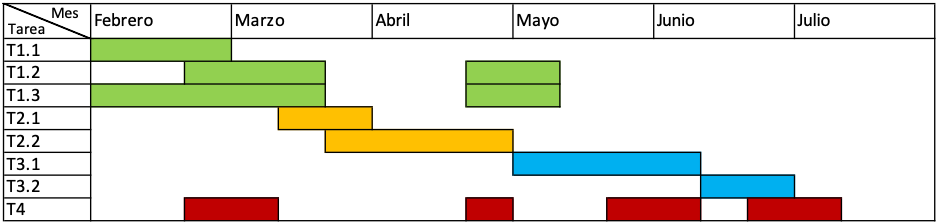
\includegraphics[scale=0.38]{imagenes/gantt.png}}  
    \caption{Diagrama de Gantt con la temporización de las tareas.} \label{fig:figura1}
\end{figure}

\section{Gestión de recursos}

\subsection{Recursos humanos}
\noindent El proyecto cuenta con dos personas trabajando sobre él:
\begin{itemize}
    \item \textbf{Rocío Romero Zaliz.} Profesora del Departamento de Ciencias de la Computación e Inteligencia Artificial tutora del proyecto. Encargada de supervisar al alumno, guiando su trabajo y aconsejándole cuando lo necesite. Se reunirá con él de forma periódica para comentar los avances e indicar posibles pasos a seguir.
    \item \textbf{Pedro Bedmar López.} Estudiante del Grado en Ingeniería Informática que realiza el TFG. Se encargará de su desarrollo y de la elaboración de la memoria.
\end{itemize}

\subsection{Recursos materiales}

Una ventaja del sector tecnológico es que muchos proyectos no necesitan una gran infraestructura para llevarse a cabo. En este caso se hace uso de lo siguiente:
\begin{itemize}
    \item \textbf{Ordenador personal.} Equipo desde el que trabajará el estudiante. Lo utilizará para consultar la literatura, implementar el código y redactar la memoria. En concreto, se trata de un MacBook Pro 15' 2015, que monta un procesador Intel Core i7 a 2.5 GHz y 16 GB de RAM.
    \item \textbf{Monitor.} Utilizado como apoyo a la pantalla del portátil. El modelo utilizado ha sido fabricado por la marca Benq, y presenta una resolución 1920x1080.
    \item \textbf{Clúster GPU.} Hoy en día, la mayoría del entrenamiento de modelos en Aprendizaje Automático y Deep Learning no se lleva a cabo de forma local, sino en un clúster habilitado para ello. La Universidad de Granada, y en concreto el Instituto DaSCI (Instituto Andaluz Interuniversitario en Data Science and Computational Intelligence), cuenta con uno de ellos donde mediante SLURM se pueden enviar trabajos que se ejecutaran en una GPU, acelerando en gran medida los entrenamientos.
\end{itemize}

\subsection{Recursos software}
\noindent Se utilizan distintos programas que apoyan en distintas tareas:
\begin{itemize}
    \item \textbf{macOS Monterey 12.3.1.} Por encima del resto de programas, se encuentra el Sistema Operativo, encargado de administrar los recursos hardware y controlar la ejecución de procesos.
    \item \textbf{PyCharm 2021.3.3.} IDE desarrollado por la compañía JetBrains, ideal para trabajar con proyectos en Python e incluso con Jupyter Notebooks. Además, se integra directamente mediante SSH con el clúster GPU, permitiendo la sincronización de ficheros entre el espacio de trabajo local y el remoto. Aunque es un software de pago, los estudiantes pueden descargarlo de forma gratuita.
    \item \textbf{Git y GitHub.} Git es un software de control de versiones que permite ir almacenando versiones intermedias del código, de forma que se puede volver hacia atrás si es necesario. También facilita el trabajo en equipo, ya que puede combinar el trabajo de múltiples personas de forma automática (siempre y cuando no hayan trabajado sobre la misma línea). GitHub es una plataforma de alojamiento de proyectos que utilizan Git. Nos es útil, ya que actúa como almacenamiento de seguridad de nuestro trabajo.
    \item \textbf{Google Meet.} Producto de videoconferencias de Google. Es la plataforma oficial de comunicación síncrona en la Universidad de Granada. Será utilizado en las reuniones entre los integrantes del equipo.
    \item \textbf{VSCode y \LaTeX.} VSCode es un editor de código desarrollado por Microsoft. Cuenta con multitud de extensiones creadas por la comunidad, entre ellas destacan algunas que permiten el formateo y compilado de ficheros \LaTeX. Este software es un sistema de composición de textos utilizado para escribir esta memoria.
\end{itemize}

\section{Presupuesto}
En esta sección se presenta el presupuesto del proyecto.

\subsection{Coste de recursos humanos}
La mayor parte del coste vendrá generado por las horas de trabajo dedicadas al proyecto por el alumno.

Según la Universidad Europea, el salario medio de un informático recién egresado ronda los 18000 - 22000€ al año \cite{salario_ue}. Si contamos el número de días hábiles para este año 2022, obtenemos 253 días \cite{dias_laborables}, a los que hay que restarle 22 días de vacaciones \cite{vacaciones}. En total trabajaría 231 días al año ocho horas por día, lo que hace un total de 1848 horas. Si tomamos como salario medio los 20000 euros anuales y los dividimos por el número de horas que se trabajan al año, obtenemos un coste por hora de 10.82€.

\subsection{Otros costes}
A la cantidad total hay que añadirle los impuestos y tasas correspondientes, en nuestro caso el IVA (21\%). En mi caso, por ser mi primer año como autónomo, el tipo de IRPF que me corresponde es del 7\%.

\subsection{Presupuesto final}

El presupuesto queda desglosado en la tabla inferior, siendo el importe total a percibir 3700.44€.

\begin{table}[H]
\begin{tabular}{@{}llll@{}}
\toprule
\textbf{Artículo}        & \textbf{Coste (€)} & \textbf{Cantidad}      & \textbf{Importe} \\ \midrule
Hora de trabajo autónomo & 10.82€             & 300                    & 3246€            \\
                            &                    &                        &                  \\
                            &                    &                        &                  \\ \midrule
\textbf{Base imponible:} &                    & \textbf{}              & 3246€            \\
                            &                    & \textbf{IVA 21\%}      & 681.66€          \\
                            &                    & \textbf{Ret. 7\% IRPF} & 227.22€          \\ \midrule
\textbf{Total:}          &                    &                        & 3700.44€        
\end{tabular}
\end{table}